% ── Capítulo 4: Planteamiento de la comparativa ──────────────────────────────
\chapter{Planteamiento de la comparativa}
\label{cap:planteamiento}

El presente capítulo describe el trabajo previo realizado para definir el diseño experimental de la comparativa, incluyendo la selección y caracterización del conjunto de datos, la identificación de las arquitecturas a evaluar, los criterios de éxito adoptados, las métricas de evaluación y el protocolo de validación temporal que garantiza la validez metodológica de los resultados. Las decisiones aquí documentadas son la concreción operativa de los objetivos específicos formulados en el Capítulo~\ref{cap:objetivos} y el punto de partida necesario para interpretar correctamente los resultados que se presentan en el Capítulo~\ref{cap:resultados}.

\section{Identificación del problema y trabajo previo}
\label{sec:trabajo_previo}

El problema central que motiva esta comparativa ---documentado en los capítulos anteriores--- es la ausencia de marcos de evaluación cuantitativos que permitan seleccionar modelos de pronóstico en entornos de FP\&A con base en criterios objetivos y reproducibles. Para abordarlo de forma rigurosa, el trabajo previo consistió en tres actividades: una revisión sistemática de la literatura para identificar las familias de modelos con mayor representación en benchmarks comparativos de series temporales financieras; un análisis exploratorio del conjunto de datos seleccionado para caracterizar las series disponibles y determinar los parámetros del experimento; y la definición del protocolo de validación temporal que garantiza la comparabilidad de los resultados.

La revisión de la literatura ---desarrollada en detalle en el Capítulo~\ref{cap:contexto}--- permitió identificar cuatro familias de modelos que representan niveles de complejidad algorítmica bien diferenciados. Esta taxonomía de complejidad creciente estructura el diseño del experimento: no se busca evaluar el mayor número posible de modelos, sino representar cada nivel con los algoritmos más representativos de su familia, de modo que los resultados permitan extraer conclusiones sobre la relación entre complejidad y valor en FP\&A.

El análisis exploratorio del conjunto de datos reveló una heterogeneidad considerable en la longitud de las series disponibles. Esta variabilidad tiene implicaciones directas para el diseño del protocolo de backtesting: series demasiado cortas no proporcionan suficientes iteraciones walk-forward para analizar la estabilidad temporal del desempeño. El umbral de 72 meses como longitud mínima de inclusión responde precisamente a esta consideración, garantizando al menos cuatro iteraciones de evaluación independientes bajo el protocolo adoptado.

\section{Descripción del conjunto de datos}
\label{sec:dataset}

La selección del conjunto de datos M4 Financial Monthly responde a tres criterios. En primer lugar, su origen en una competición de pronóstico de referencia internacional garantiza que las series han sido sometidas a un proceso de \textit{curation} y que los resultados son comparables con los de otros estudios que utilizan el mismo benchmark \parencite{Makridakis2020M4}. En segundo lugar, la categoría financiera mensual es la más representativa del contexto de FP\&A en términos de frecuencia temporal y naturaleza de las variables. En tercer lugar, el volumen de series disponibles tras el filtrado permite obtener estimaciones de desempeño estadísticamente robustas y analizar el comportamiento de los modelos en distintos segmentos. La Tabla~\ref{tab:dataset} recoge las características principales del conjunto de datos.

\begin{table}[H]
\caption{\textbf{Tabla 7.} \textit{Características del conjunto de datos M4 Financial Monthly utilizado en la comparativa.}}
\label{tab:dataset}
\vspace{4pt}
\begin{tabular}{>{\raggedright\arraybackslash}p{4cm} >{\raggedright\arraybackslash}p{9.5cm}}
\toprule
\textbf{Dimensión} & \textbf{Descripción} \\
\midrule
Fuente & M4 Competition Dataset, categoría Financial Monthly \parencite{Makridakis2020M4}. Conjunto de acceso público diseñado específicamente para el benchmarking de modelos de pronóstico. \\
Series originales disponibles & 10.987 series temporales financieras mensuales. \\
Criterio de filtrado aplicado & Se retienen únicamente las series con longitud real $\geq 72$ meses (6 años), umbral mínimo para garantizar suficiente historial de entrenamiento. \\
Series retenidas tras filtrado & 8.493 series (77,3\,\% del total original). \\
Frecuencia temporal & Mensual. Cada observación corresponde a un período de un mes. \\
Longitud de las series (tras filtrado) & Media: 184 meses $\cdot$ Mediana: 175 meses $\cdot$ P25: 74 meses $\cdot$ P75: 237 meses $\cdot$ Máximo: 1.502 meses. \\
Horizonte de pronóstico & 18 meses. Corresponde al horizonte estándar M4 mensual y representa aproximadamente un ciclo y medio de planificación financiera anual. \\
Naturaleza de las series & Series de variables económicas y financieras diversas (ingresos, indicadores macroeconómicos, métricas corporativas). Las series no están etiquetadas por tipo de cuenta contable. \\
\bottomrule
\end{tabular}
\vspace{4pt}

\small\textit{Fuente: elaboración propia a partir del M4 Competition Dataset \parencite{Makridakis2020M4}.}
\end{table}

\textbf{Limitación relevante.} Las series del M4 no están etiquetadas por tipo de cuenta contable, lo que impide el análisis de contribución al error por categoría contable en el sentido estricto que se plantea en la literatura de FP\&A. Como alternativa metodológica, el análisis desagregado se realiza por decil de volumen absoluto de la serie, que es un proxy razonable del impacto financiero relativo de cada error de pronóstico. Esta decisión queda documentada como una limitación del trabajo y como una línea de extensión futura con datos de origen organizacional real.

\textbf{Submuestra estratificada.} Dado que el protocolo walk-forward con múltiples modelos estadísticos (incluido SARIMA con selección automática de parámetros) es computacionalmente inviable sobre las 8.493 series completas en un entorno de CPU, el experimento se ejecuta sobre una submuestra estratificada de $N = 400$ series seleccionadas mediante muestreo aleatorio estratificado por cuartil de longitud, con semilla fija (\texttt{SEED = 42}). Esta decisión garantiza: (1) que todos los modelos compiten sobre exactamente las mismas series y los mismos \textit{folds} (comparación justa); (2) la reproducibilidad total del experimento; y (3) la representatividad de los distintos perfiles de longitud presentes en el dataset completo.

\section{Modelos incluidos en la comparativa}
\label{sec:modelos_comparativa}

La selección de modelos sigue la taxonomía de complejidad creciente presentada en el Capítulo~\ref{cap:contexto}. Para cada nivel se ha seleccionado el algoritmo más representativo con base en su presencia en la literatura de benchmarking y en la disponibilidad de implementaciones maduras y reproducibles en Python. La Tabla~\ref{tab:modelos_seleccion} describe los seis modelos incluidos.

\begin{table}[H]
\caption{\textbf{Tabla 8.} \textit{Modelos incluidos en la comparativa: nivel de complejidad, implementación y justificación.}}
\label{tab:modelos_seleccion}
\vspace{4pt}
\small
\begin{tabular}{>{\raggedright\arraybackslash}p{1.8cm} >{\raggedright\arraybackslash}p{2.4cm} >{\raggedright\arraybackslash}p{2.6cm} >{\raggedright\arraybackslash}p{3.4cm} >{\raggedright\arraybackslash}p{3.4cm}}
\toprule
\textbf{Nivel} & \textbf{Modelo} & \textbf{Librería} & \textbf{Estrategia} & \textbf{Justificación} \\
\midrule
Baseline & Seasonal Naïve & NumPy (propia) & Repite el patrón estacional de los últimos 12 meses & Referencia mínima obligatoria \parencite{Hyndman2021} \\
Estadístico & ETS & statsforecast (AutoETS) & Selección automática por AICc & Estándar FP\&A; estado actual de la práctica \parencite{Armstrong2001} \\
Estadístico & Holt-Winters & statsmodels & Variante aditiva o multiplicativa seleccionada por los datos & Versión extendida con estacionalidad explícita \parencite{Hyndman2021} \\
Estadístico & SARIMA & statsforecast (AutoARIMA) & Algoritmo Hyndman-Khandakar; orden seleccionado por AICc & Modelo univariado con estacionalidad de referencia \parencite{Hyndman2021} \\
ML & LightGBM & lightgbm & Global forecasting tabular; 36 lags; predicción recursiva & Mejor resultado de gradient boosting en M4/M5 \parencite{Januschowski2020} \\
DL & MLP Bottleneck & PyTorch & Global; direct forecasting 18 pasos; BatchNorm + AdamW & Evalúa si DL tabular supera al gradient boosting \parencite{LimZohren2021} \\
DL & N-BEATS & PyTorch (propia) & Global; direct; bloques de tendencia y estacionalidad & Arquitectura nativa de series temporales con interpretabilidad estructural \parencite{Oreshkin2020} \\
\bottomrule
\end{tabular}
\normalsize
\vspace{4pt}

\small\textit{Fuente: elaboración propia.}
\end{table}

Una aclaración metodológica relevante afecta a los modelos de \textit{machine learning} y \textit{deep learning}: ambos se implementan bajo el paradigma de \textit{global forecasting}, es decir, un único modelo entrenado simultáneamente con todas las series disponibles, tratando cada ventana temporal de cada serie como una muestra independiente. Este enfoque permite que los modelos aprendan patrones compartidos entre series, lo que ha demostrado ser especialmente ventajoso cuando el número de series es grande \parencite{Januschowski2020}. La comparación entre modelos locales (Seasonal Naïve, ETS, Holt-Winters, SARIMA) y modelos globales (LightGBM, MLP, N-BEATS) es, en sí misma, una de las dimensiones de análisis del experimento.

\section{Métricas de evaluación}
\label{sec:metricas_evaluacion}

La selección de métricas responde al principio establecido en el Capítulo~\ref{cap:contexto}: la evaluación debe operar en dos planos complementarios. Las métricas estadísticas permiten comparar la precisión técnica de forma independiente de la escala y el dominio. Las métricas de impacto económico traducen esa precisión en términos de valor para el negocio. La Tabla~\ref{tab:metricas_seleccion} describe las seis métricas adoptadas.

\begin{table}[H]
\caption{\textbf{Tabla 9.} \textit{Métricas de evaluación adoptadas: categoría, nivel de análisis y rol en la comparativa.}}
\label{tab:metricas_seleccion}
\vspace{4pt}
\begin{tabular}{>{\raggedright\arraybackslash}p{2.5cm} >{\raggedright\arraybackslash}p{2.8cm} >{\raggedright\arraybackslash}p{2.5cm} >{\raggedright\arraybackslash}p{5.5cm}}
\toprule
\textbf{Métrica} & \textbf{Categoría} & \textbf{Nivel de análisis} & \textbf{Rol en la comparativa} \\
\midrule
MAE & Error absoluto & Por serie $\cdot$ Global & Error en unidades originales; intuición directa del analista \\
RMSE & Error cuadrático & Por serie $\cdot$ Global & Sensibilidad a errores grandes; penaliza outliers \\
MAPE & Error porcentual & Por serie $\cdot$ Global & Comunicación a equipos de negocio; complementa al sMAPE \\
sMAPE & Error porcentual simétrico & Por serie $\cdot$ Global & Métrica principal; estándar M4; permite comparar con literatura \parencite{Petropoulos2022} \\
MASE & Error escalado & Por serie $\cdot$ Global & Comparación robusta frente al naïve estacional; valores $<1$ indican superación del baseline \parencite{Hyndman2021} \\
WAPE & Impacto económico & Agregado $\cdot$ Por decil & Pondera errores por volumen; alinea la medición con el impacto real en el negocio \parencite{Makridakis2022} \\
\bottomrule
\end{tabular}
\vspace{4pt}

\small\textit{Fuente: elaboración propia a partir de \textcite{Petropoulos2022}, \textcite{Hyndman2021} y \textcite{Makridakis2022}.}
\end{table}

La elección del sMAPE como métrica principal de comparación responde a su condición de estándar en la competición M4, lo que permite contrastar los resultados de este trabajo con los reportados en la literatura de referencia. Sin embargo, el análisis no se limita a esta métrica: el MASE completa la perspectiva estadística con una referencia explícita al modelo naïve estacional, mientras que el WAPE introduce la dimensión económica que diferencia el enfoque de este trabajo. Esta combinación permite responder a preguntas distintas: ¿qué modelo comete menos error en promedio?, ¿qué modelo supera de forma más consistente al baseline simple?, y ¿qué modelo reduce el error donde el impacto financiero es mayor?

\section{Protocolo de validación temporal}
\label{sec:protocolo_wf}

El protocolo de backtesting walk-forward es el componente metodológico más crítico de la comparativa. Como demostraron \textcite{Bergmeir2012}, la alternativa más común ---el hold-out simple con un único período de test fijo--- produce estimaciones de desempeño entre un 20\,\% y un 30\,\% más optimistas que los resultados reales en producción. La Tabla~\ref{tab:protocolo} documenta los parámetros del protocolo y su justificación.

\begin{table}[H]
\caption{\textbf{Tabla 10.} \textit{Parámetros del protocolo de backtesting walk-forward y su justificación.}}
\label{tab:protocolo}
\vspace{4pt}
\begin{tabular}{>{\raggedright\arraybackslash}p{4.5cm} >{\raggedright\arraybackslash}p{9cm}}
\toprule
\textbf{Parámetro} & \textbf{Valor y justificación} \\
\midrule
Ventana mínima de entrenamiento & 54 meses (4,5 años). Garantiza al menos cuatro ciclos estacionales completos para el ajuste de parámetros \parencite{Hyndman2021}. \\
Horizonte de pronóstico & 18 meses. Estándar M4 mensual; cubre aproximadamente un ciclo y medio de planificación financiera. \\
Desplazamiento entre iteraciones & 12 meses. Cada nueva ventana avanza un año completo, preservando la estructura estacional de los datos. \\
Variante de ventana & Expanding window (ventana creciente). El entrenamiento acumula todas las observaciones disponibles hasta el punto de corte de cada iteración. Apropiado dado que las series no presentan cambios de régimen conocidos. \\
Iteraciones por serie & Variable según longitud. Para una serie de longitud media (184 meses), se generan aproximadamente 9 iteraciones de evaluación independientes. \\
Control de fuga de datos & En ninguna iteración los datos del período de evaluación ($t+1$ a $t+18$) son accesibles durante el ajuste del modelo ni durante la ingeniería de \textit{features}. Verificado automáticamente por el módulo \texttt{verify\_no\_leakage} \parencite{Bergmeir2012}. \\
\bottomrule
\end{tabular}
\vspace{4pt}

\small\textit{Fuente: elaboración propia a partir de \textcite{Bergmeir2012} y \textcite{Hyndman2021}.}
\end{table}

Las métricas finales reportadas en el Capítulo~\ref{cap:resultados} corresponden a la media y la desviación estándar de todas las iteraciones walk-forward de todas las series de la submuestra, lo que produce estimaciones representativas del desempeño esperado en condiciones de producción real y permite cuantificar la estabilidad temporal de cada modelo. La Figura~\ref{fig:walkforward_schema} ilustra el esquema de cuatro iteraciones representativas de este protocolo.

\begin{figure}[H]
\caption{\textbf{Figura 1.} \textit{Esquema de validación walk-forward con ventana creciente (\textit{expanding window}). Cada fila representa un fold; el área azul corresponde al conjunto de entrenamiento y el área roja al horizonte de evaluación de 18 meses.}}
\label{fig:walkforward_schema}
\vspace{4pt}
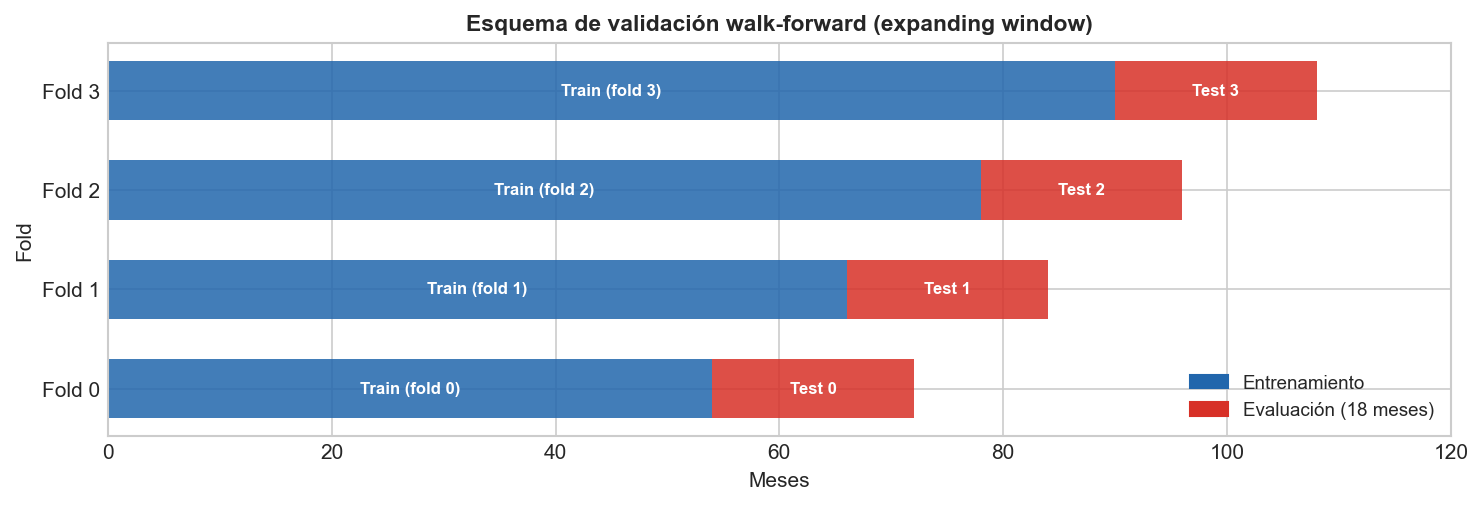
\includegraphics[width=\textwidth]{../results/figures/fig01_walk_forward_schema.png}
\vspace{4pt}

\small\textit{Fuente: elaboración propia. El desplazamiento entre iteraciones es de 12 meses (step); la ventana de entrenamiento crece acumulando todas las observaciones históricas disponibles hasta el punto de corte de cada fold.}
\end{figure}

\section{Criterios de éxito}
\label{sec:criterios_exito}

Para que la comparativa produzca conclusiones operacionalizables y no simplemente un ranking de modelos, es necesario definir con antelación qué condiciones constituyen un resultado significativo. Los criterios de la Tabla~\ref{tab:criterios} operan en dos niveles: cuándo un modelo supera al baseline, y cuándo la mejora de un modelo complejo sobre otro justifica la inversión adicional en complejidad.

\begin{table}[H]
\caption{\textbf{Tabla 11.} \textit{Criterios de éxito de la comparativa: condiciones de superación del baseline y de diferenciación entre modelos.}}
\label{tab:criterios}
\vspace{4pt}
\begin{tabular}{>{\raggedright\arraybackslash}p{2.5cm} >{\raggedright\arraybackslash}p{5.5cm} >{\raggedright\arraybackslash}p{5.5cm}}
\toprule
\textbf{Criterio} & \textbf{Condición de superación del baseline} & \textbf{Condición de diferenciación entre modelos complejos} \\
\midrule
sMAPE global & Reducción $\geq 1$ pp absoluto respecto al Seasonal Naïve (referencia: 14,45\,\%) & Reducción estadísticamente consistente entre iteraciones walk-forward \\
MASE global & MASE $< 1{,}0$ para todos los modelos evaluados & MASE $< 0{,}90$ para los modelos de mayor complejidad \\
WAPE & El WAPE de cualquier modelo no supera el WAPE del baseline en el 30\,\% de mayor volumen & Reducción del WAPE en los deciles de mayor volumen a medida que aumenta la complejidad \\
Estabilidad temporal & CV del sMAPE entre iteraciones walk-forward $< 25\,\%$ para todos los modelos & Los modelos complejos no muestran deterioro significativo en las iteraciones más recientes \\
\bottomrule
\end{tabular}
\vspace{4pt}

\small\textit{Fuente: elaboración propia. El valor de referencia del Seasonal Naïve (14,45\,\%) se obtuvo en la fase exploratoria del experimento sobre la submuestra estratificada.}
\end{table}

Estos criterios no son umbrales absolutos derivados de la teoría, sino referencias operativas construidas a partir de los resultados reportados en benchmarks comparables \parencite{Makridakis2022}. El criterio de estabilidad temporal merece una mención específica porque responde a una necesidad propia del contexto de FP\&A que los benchmarks convencionales rara vez abordan: en un entorno de planificación financiera, un modelo que produce estimaciones excelentes durante algunos períodos pero se deteriora significativamente en otros tiene un valor práctico limitado, porque los analistas no pueden confiar en él de forma sistemática.
